\begin{figure}[htb]
    % \vspace{-0.1cm}
    \begin{center}
    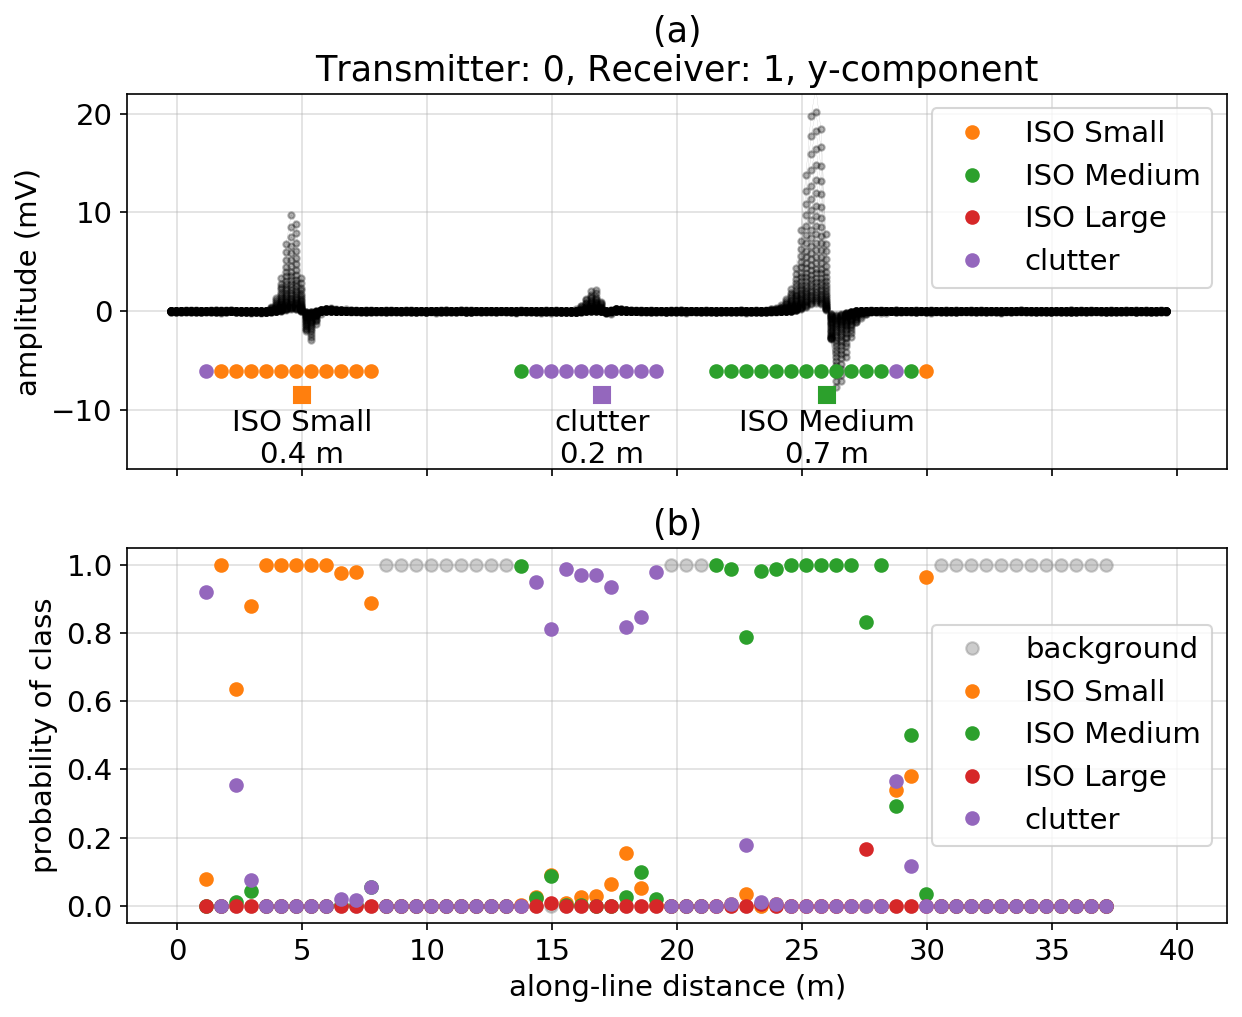
\includegraphics[width=\columnwidth]{figures/profile-line.png}
    \end{center}
    % \vspace{-0.5cm}
\caption{
    (a) Simulated UltraTEM data collected along a profile line (black) with 3 items whose along-line location is indicated by the squares.
    The number indicated beneath each item indicates its depth.
    The colored circles denote the classification obtained from the trained neural network for signal within a 3m window that is centered at the along-line location of the circle.
    (b) Probabilities associated with each class.
}
\label{fig:profile-line}
% \vspace{-0.1cm}
\end{figure}
